

\section{Results}

\subsection{Position depdendence}

In this section, we present results for. We begin by motivating choices for nominal conditions for the position of the laser beam and the laser power. Figure \ref{fig:pos_dependence} shows the MWS signal as a function of the position of the laser beam. 

We observe that near the exit of the torch there is a signficant fluctuation in the $AS$ signal in the absence of a laser pulse. We discuss the source of this fluctuation in the discussion or SI. For the present discussion, the important point is that these fluctuations are signficant compared to the signal induced by the laser pulse, and they therefore preclude accurate measurement of the time decay of the AS signal. 

In Figure \ref{fig:pos_dependence}B the we quantify the signal to fluctuation ratio to find the optimal position for the MWS diagnostic. We define the signal as the maximum of the AS signal ($AS_{max}$) within a microsecond of the laser pulse, and the fluctuation as the standard deviation of the AS signal in the time prior to the laser pulse ($PP_{std}$). We observe that both $AS_{max}$ and $PP_{std}$ increase until about 100 mm downstream from the torch, and then decrease. However, $PP_{std}$ decreases more rapidly than $AS_{max}$, so the signal to fluctuation ratio increases to a maximum at approximately 180 mm downstream from the torch. This distance defined the nominal position for the MWS diagnostic.


\begin{figure}[h]
    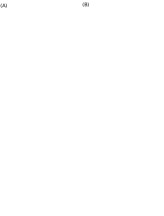
\includegraphics[width=0.8\linewidth]{\repodir/figures/output/MWS_Position.png} 
    \caption{Position dependence of the MWS signal}
    \label{fig:pos_dependence}
\end{figure}

\subsection{Laser power dependence}

Figure \ref{fig:power_dependence} shows the MWS signal as a function of the laser power. We observe that the AS signal increases superlinearly with the laser power. 

\begin{figure}[h]
    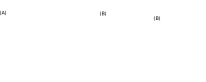
\includegraphics[width=0.8\linewidth]{\repodir/figures/output/MWS_Power.png} 
    \caption{Power dependence}
    \label{fig:power_dependence}
\end{figure}


\subsection{K dependence}

\begin{figure}[h]
    \includegraphics[width=0.8\linewidth]{\repodir/experiment/analysis/tcs/output/figures/53x_params.png} 
    \caption{Kwt dependence}
    \label{fig:kwt_dependence}
\end{figure}


\subsection{Cantera}

\begin{figure}[h]
    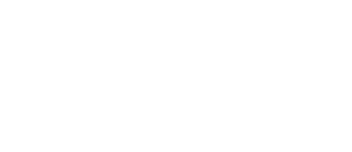
\includegraphics[width=\linewidth]{\repodir/figures/output/Cantera_alpha.png} 
    \caption{Cantera Alpha results}
\end{figure}
